\textbf{A.3.1. Input data.} I measure the body coordinate $u(t)$ and road coordinate $u_b(t)$ upward from static equilibrium. The spring and damper act through their relative deformation, so the wheel displacement is the excitation input. The supplied diagram therefore represents base displacement excitation rather than an applied force.

{\begin{center}\small\begin{tabular}{@{}lrl@{}}
\toprule\noalign{}
Quantity & Value & Unit \\
\midrule\noalign{}
$a$ & 0.1524 & m \\
$\lambda$ & 42.672 & m \\
$f_n$ & 0.960 & Hz \\
$\zeta$ & 0.140 & 1 \\
$v_{\max}$ & 50.5155 & m/s \\
$N_\lambda$ & 2 & wavelengths \\
$N_f$ & 2000 & points \\
$|H|_{\mathrm{lim}}$ & 1.50 & 1 \\
\bottomrule\end{tabular}\end{center}}

For the equations of motion, the spring and damper forces depend on $u-u_b$ and $\dot u-\dot u_b$. Newton's law consequently gives
\[
m\ddot u+c(\dot u-\dot u_b)+k(u-u_b)=0,
\qquad
m\ddot u+c\dot u+ku=c\dot u_b+ku_b.
\]
With $\omega_n=\sqrt{k/m}$ and $c/m=2\zeta\omega_n$, harmonic inputs $u_b=\Re\{\hat U_b e^{i\omega t}\}$ give the absolute body-to-road displacement ratio
\[
H(r)=\frac{\hat U}{\hat U_b}
=\frac{1+i2\zeta r}{1-r^2+i2\zeta r},
\qquad r=\frac{f}{f_n}.
\]
Its magnitude is
\[
|H(r)|=\sqrt{\frac{1+(2\zeta r)^2}{(1-r^2)^2+(2\zeta r)^2}}.
\]
The numerator follows from the base-motion terms on the right side of the equation of motion. It is also the absolute displacement transmissibility derived in the course notes (pp. 56--59).

\textbf{A.3.2. Wavy-road wavenumber.} One spatial period advances the phase by $2\pi$, so
\[
\gamma=\frac{2\pi}{\lambda}
=\frac{2\pi}{42.672\ \mathrm{m}}
=0.147244\ \mathrm{rad/m}.
\]
\[\boxed{\gamma=0.1472\ \mathrm{rad/m}}\qquad\text{(A.3.2)}\]

\textbf{A.3.3. Road profile.} The supplied cosine starts at a crest, hence $u_b(x)=a\cos(\gamma x)$. The following figure spans the requested two wavelengths, or $85.344\ \mathrm{m}$.
\begin{figure}[H]
\centering
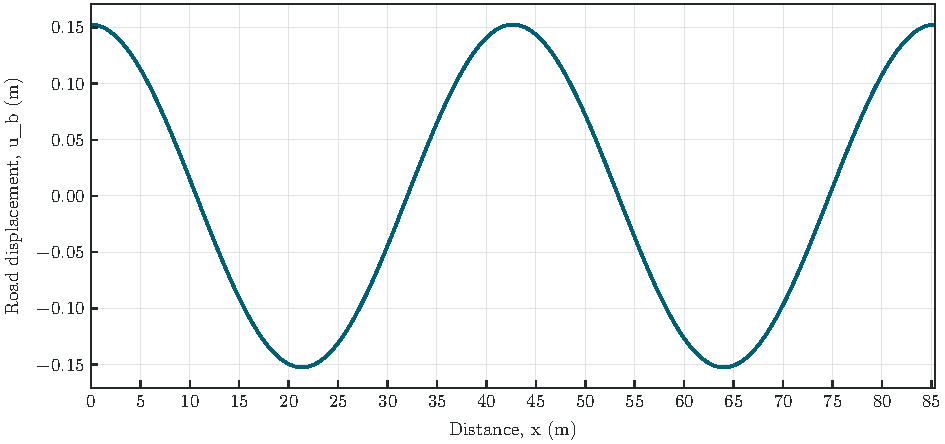
\includegraphics[width=0.90\linewidth]{figures/generated/solutions/A3-road.pdf}
\caption{A.3.3. Cosine road profile across two wavelengths.}
\end{figure}
\[\boxed{u_b(x)=0.1524\cos\!\left(\frac{2\pi x}{42.672\ \mathrm{m}}\right)\ \mathrm{m},\quad 0\leq x\leq85.344\ \mathrm{m}}\qquad\text{(A.3.3)}\]

\textbf{A.3.4. Road-frequency range.} At constant speed, $x=vt$ makes the road input $u_b(t)=a\cos(2\pi vt/\lambda)$, so $f=v/\lambda$. The maximum road frequency is therefore
\[
f_{\max}=\frac{v_{\max}}{\lambda}
=\frac{50.5155\ \mathrm{m/s}}{42.672\ \mathrm{m}}
=1.18381\ \mathrm{Hz}.
\]
I evaluate $f=\operatorname{linspace}(0,1.18381\ \mathrm{Hz},2000)$ for the plotted curves.
\[\boxed{f_{\max}=1.184\ \mathrm{Hz},\qquad N_f=2000}\qquad\text{(A.3.4)}\]

\textbf{A.3.5. Healthy-shock frequency response.} The figure plots the absolute body displacement transmissibility for healthy shocks. The matched-frequency marker is evaluated at exactly $f=f_n$, while the peak marker is evaluated at the analytic stationary point; neither marker is restricted to the sampled curve grid.
\begin{figure}[H]
\centering
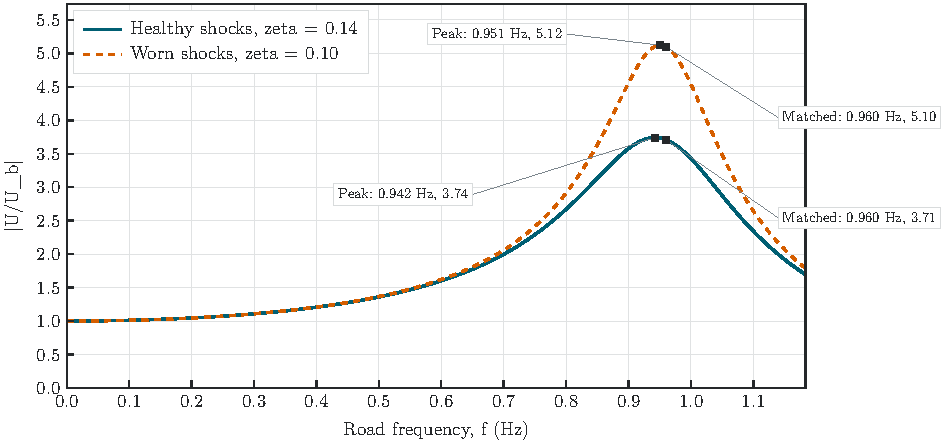
\includegraphics[width=0.94\linewidth]{figures/generated/solutions/A3-frequency.pdf}
\caption{A.3.5 and A.3.10. Absolute body-to-road displacement FRF versus road frequency. The curves compare healthy and worn shocks; square markers show analytic peak and matched-frequency events.}
\end{figure}

\textbf{A.3.6. Matched-frequency response.} At $r=1$, the complex response is $H(1)=1-i/(2\zeta)$, and its magnitude is
\[
|H_n|=\sqrt{1+\frac{1}{(2\zeta)^2}}
=\sqrt{1+\frac{1}{(0.280)^2}}=3.70879.
\]
The 2000-point sampled curve gives $|H|=3.70894$ at its nearest sample, while the analytic matched value is $3.70879$. For comparison, the true healthy maximum is $3.74053$ at $f=0.942367\ \mathrm{Hz}$, below $f_n$.
\[\boxed{\begin{aligned}
|H_n|&=3.71\quad\text{at }f=f_n=0.960\ \mathrm{Hz},\\
|H|_{\max}&=3.74\quad\text{at }f=0.942\ \mathrm{Hz}.
\end{aligned}}\qquad\text{(A.3.6)}\]

\textbf{A.3.7. Matched-frequency speed.} Since $f=v/\lambda$, setting $f=f_n$ gives
\[
v_n=f_n\lambda=(0.960\ \mathrm{Hz})(42.672\ \mathrm{m})
=40.9651\ \mathrm{m/s}=91.6364\ \mathrm{mph}.
\]
\[\boxed{v_n=41.0\ \mathrm{m/s}=91.6\ \mathrm{mph}}\qquad\text{(A.3.7)}\]

\textbf{A.3.8. Speed response and amplification limit.} The speed sweep uses 2000 equally spaced values from $0$ to $50.5155\ \mathrm{m/s}$, with $f=v/\lambda$. The analytic event values are reported separately from the sampled graph readings.
\begin{figure}[H]
\centering
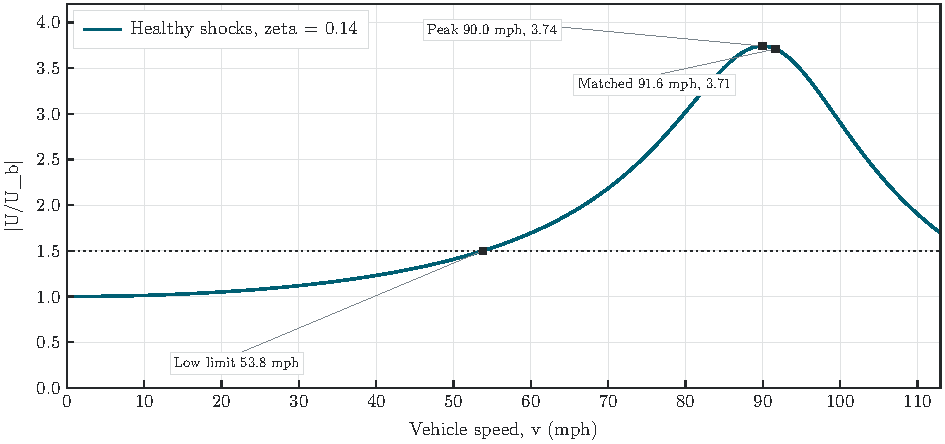
\includegraphics[width=0.94\linewidth]{figures/generated/solutions/A3-speed-healthy.pdf}
\caption{A.3.8. Healthy-shock absolute body-to-road displacement FRF versus vehicle speed. The dotted line is the 1.5 amplification threshold; square markers show analytic peak, matched-frequency, and in-range crossing events.}
\end{figure}
\begin{figure}[H]
\centering
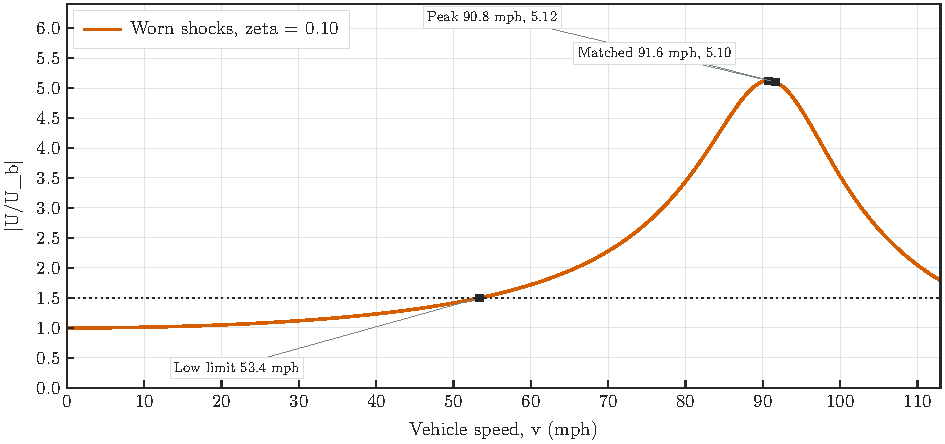
\includegraphics[width=0.94\linewidth]{figures/generated/solutions/A3-speed-worn.pdf}
\caption{A.3.10. Worn-shock absolute body-to-road displacement FRF versus vehicle speed. The dotted line is the 1.5 amplification threshold; square markers show analytic peak, matched-frequency, and in-range crossing events.}
\end{figure}

\textbf{(a) Matched-frequency event.} The speed conversion places $f_n$ at $v_n=91.6364\ \mathrm{mph}$, and the analytic ordinates are $|H_n|=3.70879$ for healthy shocks and $|H_n|=5.09902$ for worn shocks. These agree with A.3.6 and A.3.7.

\textbf{(b) True peak event.} Differentiating $|H|^2$ with respect to $q=r^2$ gives the stationary condition
\[
4\zeta^2q^2+2q-2=0.
\]
The positive root $q=[-1+\sqrt{1+8\zeta^2}]/(4\zeta^2)$ for $\zeta=0.140$ gives $r_{\mathrm{cr}}=\sqrt{q}=0.981632$, $f_{\mathrm{cr}}=0.942367\ \mathrm{Hz}$, $v_{\mathrm{cr}}=40.2127\ \mathrm{m/s}=89.9532\ \mathrm{mph}$, and $|H_{\max}|=3.74053$. This peak precedes the matched-frequency point. For worn shocks, $r_{\mathrm{cr}}=0.990334$, $f_{\mathrm{cr}}=0.950721\ \mathrm{Hz}$, $v_{\mathrm{cr}}=40.5692\ \mathrm{m/s}=90.7506\ \mathrm{mph}$, and $|H_{\max}|=5.12277$.

\textbf{(c) Threshold crossings.} Setting $q=r^2$ and $L=1.5$ reduces $|H|=L$ to
\[
L^2q^2+\bigl[L^2(4\zeta^2-2)-4\zeta^2\bigr]q+(L^2-1)=0.
\]
There are two positive crossings for each shock condition. The first crossing is the limit encountered when accelerating from rest; the second is the speed above which amplification falls below 1.5 again. The upper crossings lie above $v_{\max}$ and are not plotted.
\[
\boxed{\begin{aligned}
\zeta=0.140:&\quad v_{\mathrm{low}}=24.1\ \mathrm{m/s}=53.8\ \mathrm{mph},\\
&\quad v_{\mathrm{high}}=52.0\ \mathrm{m/s}=116.3\ \mathrm{mph},\\
\zeta=0.100:&\quad v_{\mathrm{low}}=23.9\ \mathrm{m/s}=53.4\ \mathrm{mph},\\
&\quad v_{\mathrm{high}}=52.4\ \mathrm{m/s}=117.3\ \mathrm{mph}.
\end{aligned}}\qquad\text{(A.3.8)}\]

\textbf{A.3.9. Wavelength for a 30 mph critical speed.} The requested speed is the true peak speed, not the matched-frequency speed. Using the healthy-shock peak frequency $f_{\mathrm{cr}}=0.942367\ \mathrm{Hz}$, choose
\[
\lambda_{\mathrm{new}}=\frac{v_{\mathrm{cr,target}}}{f_{\mathrm{cr}}}
=\frac{13.4112\ \mathrm{m/s}}{0.942367\ \mathrm{Hz}}
=14.2314\ \mathrm{m}.
\]
\[\boxed{\lambda_{\mathrm{new}}=14.23\ \mathrm{m}=46.7\ \mathrm{ft}}\qquad\text{(A.3.9)}\]

\textbf{A.3.10. Worn shocks.} Repeating items (5)--(8) with $\zeta=0.100$ retains the same matched frequency $f_n=0.960\ \mathrm{Hz}$ and matched speed $v_n=91.6364\ \mathrm{mph}$, but increases the matched response to
\[
|H_n|=\sqrt{1+\frac{1}{(0.200)^2}}=5.09902.
\]
The true peak is $|H|_{\max}=5.12277$ at $f_{\mathrm{cr}}=0.950721\ \mathrm{Hz}$ and $v_{\mathrm{cr}}=40.5692\ \mathrm{m/s}=90.7506\ \mathrm{mph}$. The table compares both shock conditions. Since $|H|^2$ increases with damping ratio for $r>\sqrt{2}$, the healthy response exceeds the worn response at high frequency, even though lower damping produces a much larger resonance peak.
{\begin{center}\small\begin{tabular}{@{}lrrrr@{}}
\toprule\noalign{}
Shock condition & $|H_n|$ & $f_{\mathrm{cr}}$ (Hz) & Peak $|H|$ & $v_{\mathrm{cr}}$ (mph) \\
\midrule\noalign{}
Healthy, $\zeta=0.140$ & 3.71 & 0.942 & 3.74 & 90.0 \\
Worn, $\zeta=0.100$ & 5.10 & 0.951 & 5.12 & 90.8 \\
\bottomrule\end{tabular}\end{center}}

\[\boxed{|H_n|_{\mathrm{worn}}=5.10,\quad |H|_{\max,\mathrm{worn}}=5.12\text{ at }0.951\ \mathrm{Hz}}\qquad\text{(A.3.10)}\]

\noindent\begin{minipage}{\linewidth}\color{black}
\textbf{Graph readings.} MATLAB data tips on the 2000-point sampled curves give the readings below. The speed-grid spacing is $0.0565\,\mathrm{mph}$, so sampled extrema and threshold values differ slightly from the analytic events above.
\begin{center}\small
\begin{tabular}{@{}lrrrr@{}}
\toprule
Event & Healthy $x$ & Healthy $|H|$ & Worn $x$ & Worn $|H|$ \\
\midrule
Peak frequency (Hz) & 0.942 & 3.74 & 0.950 & 5.12 \\
Matched frequency (Hz) & 0.960 & 3.71 & 0.960 & 5.10 \\
Peak speed (mph) & 89.9 & 3.74 & 90.7 & 5.12 \\
Matched speed (mph) & 91.6 & 3.71 & 91.6 & 5.10 \\
Lower crossing (mph) & 53.8 & 1.500 & 53.4 & 1.500 \\
Upper crossing & outside sweep & -- & outside sweep & -- \\
\bottomrule
\end{tabular}
\end{center}
\end{minipage}\par
\clearpage
\matlabcaption{MATLAB calculations and direct plots for A.3.}
\lstinputlisting[style=hwmatlab]{matlab/A3.m}
